\documentclass[../manifest.tex]{subfiles}

\begin{document}

Code reviews are an essential part for modern software engineering and greatly influence software quality. Therefore, we choose to evaluate CodeStory by having participants complete two code reviews each, one with comments from our tool and one without (section \ref{eval-description}). We then analyzed the quality of the code reviews to determine if our tool had any effect in section \ref{eval-impact}. Before this study, however, we determined the general feasibility of CodeStory by performing a pilot survey among industry developers who perform code reviews on a daily basis (section \ref{eval-survey}). Threats to validity for our evaluation are described in section \ref{eval-threats}.

\subsection{Pilot Survey} \label{eval-survey}

At an early stage of this paper, we aimed to determine whether our assumption that it is useful to record developers' reasoning during coding tasks is true. Additionally, we wanted to collect information on what information may in fact be useful. We therefore collected 17 responses of industry developers who regularly perform code reviews with a survey.

After providing a brief introduction of our research, we described the following scenario: \textit{a developer has to choose a sort algorithm for a particular task. She googles "sort array in JavaScript" and finds a code snippet on StackOverflow. She copies the snippet as a scaffold into her code}.

We then let participants rate the following question on a scale of 1 (not useful) to 5 (very useful): \textit{How useful would the story above be during the code review?} The responses to this question were positive: no participant rated with 0 and only 2 participants rated with 1 (negative responses). 6 participants rated with 3 (neutral), 7 participants rated with 4 and 2 participants rated with 5 (positive). Overall, 88\% responded neutral or positive to the question whether recording the described contextual information would be useful.

Finally, we collected opinions on the particular information of interest using the same 1-to-5 scale: \textit{What elements from the above story would you consider useful?} Table~\ref{tab:elements-of-interest} shows the list of elements and the percentage of the responses that rated with either 3 (maybe useful), 4 (somewhat useful) or 5 (very useful).

Considering the majority of neutral and positive responses to our pilot survey we felt confirmed that the idea behind CodeStory is valuable and we could continue our research. The single element that had a overly negative result in the survey was the \textit{Google search query leading to StackOverflow}. We consequently chose to not include this element in the implementation of CodeStory.

\begin{table}[t]
    \centering
    \begin{threeparttable}
    \begin{tabular*}{\linewidth}{lr}
    \hline
    \textbf{Element} & \textbf{\% Ratings $\ge3$} \\
    \hline
    Google search query leading to SO & 24\% \\
    SO question URL & 76\% \\
    SO question heading & 47\% \\
    SO question content & 76\% \\
    SO answer URL & 76\% \\
    Time of access of SO page & 59\% \\
    SO answer code snippet & 53\% \\
    Entire SO answer & 47\% \\
    SO answer rating & 59\% \\
    SO answer acceptance status & 59\% \\
    SO answer comments & 59\% \\
    Other SO answers & 47\% \\
    \hline
  \end{tabular*}
  \begin{tablenotes}\footnotesize
    \item \textit{SO = StackOverflow.}
  \end{tablenotes}
  \end{threeparttable}
    \caption{Elements of interest for survey rating}
    \label{tab:elements-of-interest}
\end{table}

\subsection{Study Description} \label{eval-description}

In order to determine the usefulness of CodeStory in practice, we approached developers with code reviews. We created a bootstrap repository on Github that contained a simple Maven Java-Project. We aimed to simulate a realistic scenario where in a developer read a StackOverflow page, copied a code fragment and pasted it into their code. We chose two questions on StackOverflow as scenarios for the study:
\begin{enumerate}
  \item \textit{Gson - convert from Json to a typed ArrayList<T>}\footnote{http://stackoverflow.com/questions/12384064}
  \item \textit{How do you compare two version Strings in Java?}\footnote{http://stackoverflow.com/questions/198431}
\end{enumerate}

In (1), a developer was struggling with deserializing a JSON string to an instance of a custom Java class using the google-gson\footnote{https://github.com/google/gson} library. The developer tries to pass a class object for the generic type \code{ArrayList<JsonLog>} by passing \code{ArrayList<JsonLog>.class} to \code{fromJson} (Gson's method for deserializing a JSON string), which is not valid Java code and does not compile (because class objects cannot be created from generics that way in Java). The first answer to the question, which is also the accepted answer, describes how to solve this problem by using Gson's \code{TypeToken} class for creating the desired class object: \code{new TypeToken<List<JsonLog> >(){}.getType()}. Figure~\ref{fig:pull-request-1} shows the diff of the change that we created for this scenario.

\begin{figure}[h]
  \centering
  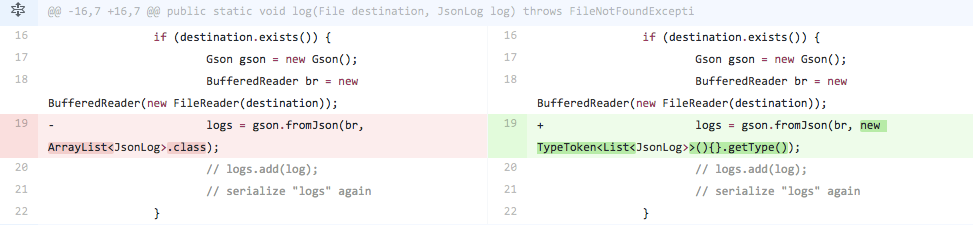
\includegraphics[width=\linewidth]{pull-request-1}
  \caption{Diff view for study scenario 1}
  \label{fig:pull-request-1}
\end{figure}

In (2), a developer was interested in how to compare version strings semantically. This question is associated with \textit{semantic versioning}\footnote{http://semver.org/} which defines what versions should be considered higher than others, i.e. \textit{1.0.0-alpha < 1.0.0-alpha.1 < 1.0.0-beta < 1.0.0-rc.1 < 1.0.0}. More specifically, the question was: \textit{given two version strings a and b, which one is higher?} For this scenario, we chose a lower ranked answer\footnote{http://stackoverflow.com/a/27891752/1105907} as a base version to be replaced by a higher ranked answer\footnote{http://stackoverflow.com/a/6640972/1105907} as the improved version. Both are answers to the given question but neither is an accepted answer. We chose to use these answers because the accepted answer did not contain any code. Figure~\ref{fig:pull-request-2} shows the diff of the change that we created for this scenario (note that this diff shows a CodeStory annotation for illustration purposes).

\begin{figure}[h]
  \centering
  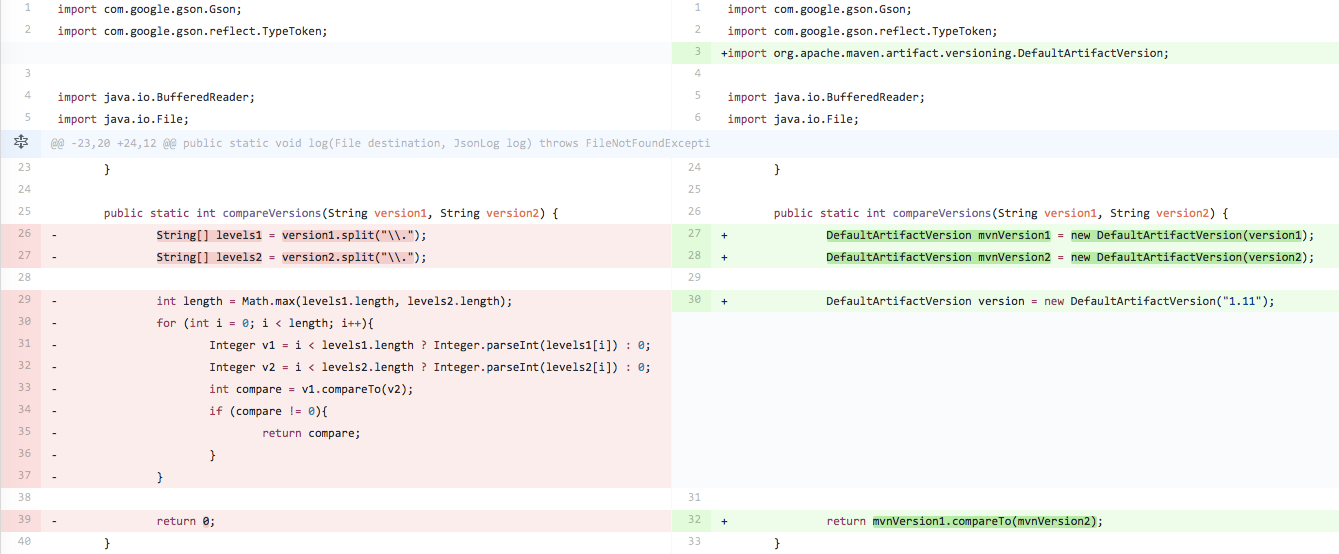
\includegraphics[width=\linewidth]{pull-request-2}
  \caption{Diff view for study scenario 2}
  \label{fig:pull-request-2}
\end{figure}

For both scenarios we now added CodeStory to the developer workflow. The resulting CodeStory pages are shown in Figures~\ref{fig:codestory-page-1} and~\ref{fig:codestory-page-2}.

\begin{figure}[h]
  \centering
  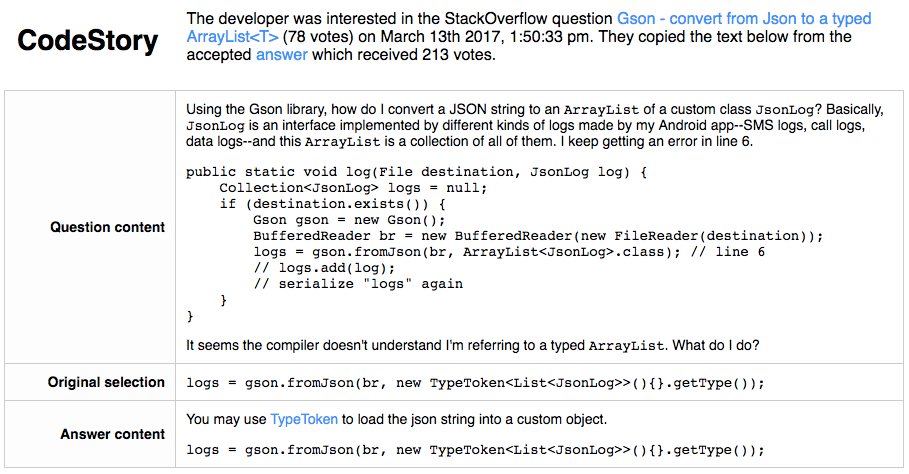
\includegraphics[width=\linewidth]{codestory-page-1}
  \caption{CodeStory page for scenario 1}
  \label{fig:codestory-page-1}
\end{figure}

\begin{figure}[h]
  \centering
  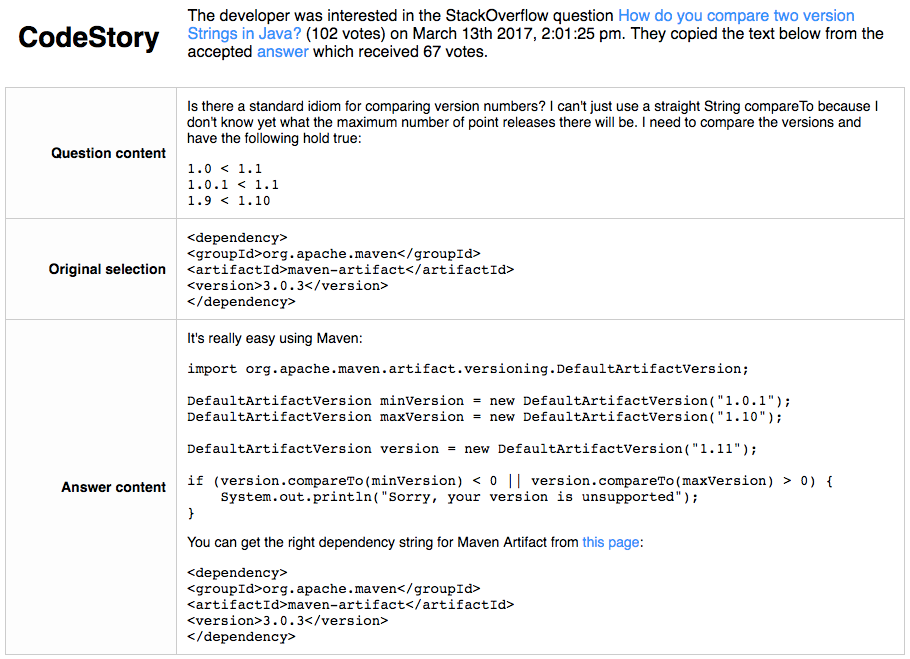
\includegraphics[width=\linewidth]{codestory-page-2}
  \caption{CodeStory page for scenario 2}
  \label{fig:codestory-page-2}
\end{figure}

For the changes described in scenarios 1 and 2, we created another version of each that included a link to the respective CodeStory page as URL in a comment above the pasted content. Since scenario 2 contained two paste operations (one in an XML file and one in a Java file), two such comments were shown in the diff.
These two scenarios resulted in four treatments for our study:
\begin{itemize}
  \item \textbf{T1:} Scenario 1 without annotation
  \item \textbf{T2:} Scenario 2 without annotation
  \item \textbf{T3:} Scenario 1 with annotation
  \item \textbf{T4:} Scenario 2 with annotation
\end{itemize}

The study was performed with 8 developers among which 4 participants were graduate students and 4 were industry developers (> 4 years of practical experience with Java). With participants from different backgrounds we ensured generalizability of our study to both academia and industry. Due to time constraints we decided to assign each participant 2 code reviews (we assumed approximately 10 minutes for each code review). To avoid learning bias for the given scenarios and treatments, we decided to let each participant do one code review for each scenario: one with annotation and one without annotation. To further avoid learning bias, we ensured that 4 participants start with a code review with annotation and the other 4 start with a code review without annotation. Table~\ref{tab:study-outline} shows the outline of treatments and participants.

\begin{table}[t]
    \centering
    \begin{tabular}{lll}
    \hline
    \textbf{Participant} & \textbf{Treatment} & \textbf{Background} \\
    \hline
    P1 & T3 + T2 & industry \\
    P2 & T3 + T2 & academia \\
    P3 & T1 + T4 & industry \\
    P4 & T1 + T4 & academia \\
    P5 & T4 + T1 & industry \\
    P6 & T4 + T1 & academia \\
    P7 & T2 + T3 & industry \\
    P8 & T2 + T3 & academia \\
    \hline
    \end{tabular}
    \caption{Study outline}
    \label{tab:study-outline}
\end{table}

For each participant we forked our bootstrap repository and created two pull requests with respect to their treatments. In the description of each pull request we asked the following questions:
\begin{itemize}
  \item \textbf{Q1:} \textit{What is the purpose of the method with the change?}
  \item \textbf{Q2:} \textit{How did the method change?}
  \item \textbf{Q3:} \textit{Why was this change made?}
\end{itemize}

We then added the participants as reviewers and instructed them to perform their code reviews in sequential order by answering our questions as comments on the pull requests. The code reviews were performed online without any further constraints.

In the instructions for the second pull request, participants were asked to complete a survey designed to determine the effectiveness of the CodeStory annotation. We first asked participants to rank their experience for each pull request on a scale from 1 (very challenging) to 5 (very easy). We then asked \textit{Was the information provided by CodeStory useful?} Table~\ref{tab:survey-results} shows the results of the survey with the ratings of each participant and the associated treatment. Finally, we gave participants the option to comment on our tool: \textit{Do you have any comments about CodeStory? Were you missing any information?}

We found two issues with our evaluation: (1) one participant (P4) did the pull requests in the opposite order and (2) another participant (P8) did not notice the CodeStory link in the diff. We consider (1) to be a minor issue that does not impact the results and (2) a major issue requiring us to \textit{ignore the results for P8} in the subsequent analysis.

\begin{table}[t]
    \centering
    \begin{threeparttable}
    \begin{tabular}{lccccr}
    \hline
    & \multicolumn{5}{c}{\textbf{Rating (1-5)}} \\
        \cline{2-6}
    \textbf{Participant} & \textbf{T1} & \textbf{T2} & \textbf{T3} & \textbf{T4} & \textbf{Overall} \\
    \hline
    P1  & - & 2 & 4 & - & 5 \\
    P2  & - & 2 & 4 & - & 5 \\
    P3  & 4 & - & - & 5 & 5 \\
    P4  & 1 & - & - & 5 & 4 \\
    P5  & 2 & - & - & 5 & 5 \\
    P6  & 3 & - & - & 5 & 5 \\
    P7  & - & 5 & 3 & - & 4 \\
    P8* & - & 4 & 2 & - & 2 \\
    \hline
    \end{tabular}
    \begin{tablenotes}\footnotesize
      \item [*] Ignored in subsequent sections because participant did not notice the CodeStory tool.
    \end{tablenotes}
    \end{threeparttable}
    \caption{Survey results}
    \label{tab:survey-results}
\end{table}

\subsection{Impact for Code Review Tasks} \label{eval-impact}

\textbf{Comparing code review comments} without (T1/T2) and with CodeStory annotation (T3/T4), we could clearly see an increase in quality using our tool. Basically, T1 and T2 induce great amounts of guessing in finding the right answers to our questions, primarily visible through phrases like "presumably", "it appears to be", "it seems to me", "I believe", etc. A decrease in quality in answers to our questions Q1-Q3 is visible for T1/T2: while Q1 could often be answered relatively easily, Q2 proved very hard and Q3 proved nearly impossible. That is why we observe the most guessing with Q3. Some participants tried to do their own online research for the questions on T1/T2 but were mostly still unable to provide good answers. Others commented that Q3 is not answerable for T1/T2. While we could generally observe higher quality answers from industry developers than from graduate students, the relationship between code reviews without and with our tool remains the same and we can therefore neglect variance resulting from participants' backgrounds.

In contrast, comments on code reviews with CodeStory (T3/T4) showed significantly higher quality. Most participants provided very good answers to our questions for these treatments. The additional contextual information provided by CodeStory clearly helped them to answer what "really happened" for the given code changed, i.e. what the developer's reasoning was during implementation. The following list provides representative examples of code review comments with answers to our questions for each treatment:

\begin{itemize}
  \item \textbf{Scenario 1 without annotation (T1):}
\textit{
Q1: I think that the method is trying to convert a json object into a gson object.
Q2: It changed through the usage of the TypedToken List and anonymous class.
Q3: The method is really small, though I believe that it was changed to consider the usage of interfaces and generics. As far as I remember, there is an issue trying to get the type of  ArrayList<JsonLog>.class and the correct implementation would have to create an anonymous class.
}
  \item \textbf{Scenario 1 with annotation (T3):}
\textit{
Q1: The purpose of the method is to parse a JSON file to an ArrayList of the custom object JsonLog. In the original version, the parsing fails because of an unconventional definition of the target Java type.
Q2: The method changed in the definition of the target type which is necessary due to Java's type safety. The type itself as well as the generic of this type are now passed on to the Json parser Gson indirectly, by first instantiating a dummy TokenType with a generic of the target type and, second, by calling .getType() on this dummy object.
Q3: The change was made because java class objects cannot simply be passed on as parameters if they are modified by generics.
}
  \item \textbf{Scenario 2 without annotation (T2):}
\textit{
Q1: Checks whether the two versions are the same.
Q2: Instead of doing a character-by-character string comparison of the two versions, converts them to a DefaultArtifactVersion object, and then compares the objects.
Q3: Hard to tell without knowing how DefaultArtifactVersion works (I could look it up but I don't want to); my guess is that the previous version is not robust to differently formatted strings that represent the same version.
}
  \item \textbf{Scenario 2 with annotation (T4):}
\textit{
Q1: The method compareVersions(a, b) determines the precedence of two version strings, a and b. Precedence is indicated by an integer return value: less-than-zero implies a < b, greater-than-zero implies a > b, and equal-to-zero implies a == b.
Q2: The implementation was changed from a homebrew implementation to an off-the-shelf implementation using Maven. Instead of comparing the versions as strings, they are now parsed into properly typed objects implementing the Comparable<T> interface.
Q3: (...) the programmer needed to implement a new feature or quirk to the version comparison logic that Maven already handles, such as comparing non-numerical version components (e.g. the "-rc1" in "1.10-rc1"), and didn't want to reinvent the wheel.
}
\end{itemize}

\textbf{Analyzing the results of the final survey} further strengthens our positive impression of CodeStory. This is most clearly visible in the comparison of the code reviews for scenario 2 (recall that we neglected the results from one participant as described in the previous section). On our scale from 1 (very challenging) to 5 (very easy), participants rated the version without annotation (T2) with 2, 2, 5 whereas all participants rated the version with annotation with 5. Scenario 1 shows similar results, though not as visible as in scenario 2. In our interpretation, this is due to the fact that the answer on StackOverflow was a simple one-liner and that question as well as answer provided far less detailed information about the problem than in scenario 2. Participants rated the version of scenario 1 without our tool (T1) with 4, 1, 2, 3 whereas they rated the version with our tool with 4, 4, 3. In summary, \textit{the average of the ratings without our tool is \textbf{2.71} while the average of the ratings with our tool is \textbf{4.43}}.

\textbf{Analyzing the optional comments of the final survey}, we noticed that one participant missed exactly the element of information that we neglected after our pilot survey, the \textit{Google search query leading to StackOverflow} (see section~\ref{eval-survey}): \textit{The search term(s) which led the programmer to that version comparison StackOverflow question could have been useful for explaining why s/he made the change. Search terms such as "java version comparison algorithm", "java version comparison best practice", and "java version comparison pre-release metadata" might all lead to that question, but convey different intents/requirements.} Our interpretation is that the participants in the pilot survey might not have fully understood what we referred to with this element and they would most likely have considered it more useful in an actual code review.

\subsection{Threads to Validity} \label{eval-threats}
While we tried to reduce the number of factors that could impact the validity of our findings there is a chance that our results may not be representative of the actual utility of CodeStory.

We evaluated the usefulness of the rationale captured by CodeStory for code review tasks. We requested participants view very short diffs in pull requests on a nearly empty bootstrap repository. This was intentional to keep the tasks short and focused but are not entirely representitive of real code reviews.

There is a potential for bias among participants and tasks. To mitigate this, we used four treatments and assigned two participants to each. One participant was from industry and the other was from academia to futher reduce bias. Additionally, to control bias among treatments, the first pull request in two of the treatments contained a CodeStory annotation while the other two had the annotation in the last pull request. In all treatments the diffs were different from each other to account for learning bias. Unfortunately, this meant that we could not directly account for variance among task but this effect should be reduced by assigning each treatment to two participants. Despite these controls and our positive results, it is possible that CodeStory would not be found favorable in general.

% \textbf{External threats}

% problems 1 and 2 described
% what is higher quality? does this really lead to higher software quality?

% does not generalize to comprehension tasks
% how we conducted the study
% does the evaluation directly answer our main question?
% bias in participants (industry vs. academic)
% interpretation of comments is subjective
% may not have captured all views/interpretations/feelings (question was just "do you consider it useful")
% scenarios are not realistic/practical/representative (generalizability) => diffs are too short and just a almost empty bootstrap repository
% did not evaluate our tool but only the "results of our tool"

\end{document}
